% Template for white paper submissions for the 
% LSST Call for Observing Strategies for DeepDrilling and Minisurveys 
% 
% The call for white papers can be found at https://github.com/lsst-pst/survey_strategy/blob/master/latex/WPcall2018.pdf
% The deadline for submissions is November 29, 2018
% Please submit your white paper via email to lsst-survey-strategy@lists.lsst.org or via a pull request on this repository 
% (https://github.com/lsst-pst/survey_strategy_wp) after creating a subdirectory named LASTNAME_FIRSTNAME_NUMBER.

% For help with white papers or the submission process, please post at http://community.lsst.org/c/sci/survey-strategy


\documentclass[12pt,letterpaper]{article}
\usepackage[top=1in,bottom=1.5in,left=1in,right=1in]{geometry}
\usepackage[utf8]{inputenc}
\usepackage{booktabs}
\usepackage{hyperref}
\usepackage{natbib}
\usepackage{amssymb,amsmath}
\usepackage{graphicx}

\title{The First Extragalactic Exoplanets --- What We Gain From High Cadence Observations of\\ the Small Magellanic Cloud?}
\author{Rados\l{}aw Poleski and Przemek Mr\'oz}
\date{November 2018}

\begin{document}

\maketitle

\begin{abstract}
We propose to increase LSST cadence for the Small Magellanic Cloud which will 
enable finding dozens of microlensing events annually and potentially, a few 
planetary events over the course of the survey.  These would be 
the first extragalactic exoplanets ever discovered and will give us a unique constraint on 
the planet formation and evolution under different environments.  We discuss what changes in 
the LSST observing strategy are required.  Presented analysis takes into account 
an extensive photometric follow-up program. 
\end{abstract}

\section{White Paper Information}
Please contact Radek Poleski, \url{radek.poleski@gmail.com}, with any questions about this white paper.  
% Please provide contact information (name and email address) of the appropriate author(s) for this white paper.
% In addition, please provide the following categorization for your white paper:
\begin{enumerate} 
\item {\bf Science Category:} Exploring the Changing Sky
% which of the four main LSST science themes are addressed? Are there other
% science programs addressed by this white paper?
% 
% Website https://www.lsst.org/science gives 4 science categories, in short: 
% DM & DE, SS, variable Sky, and MW.
\item {\bf Survey Type Category:} mini survey
% please choose one of the following possibilities: the main `wide-fast-deep'
%   survey, mini survey, Deep Drilling field, Target of Opportunity observation, Other (provide details). 
\item {\bf Observing Strategy Category:} %please choose one of the following possibilities: 
%    \begin{itemize} 
%     \item a specific observing strategy to enable specific time domain science, 
%	that is relatively agnostic to where the telescope is pointed (e.g., a science case enabled 
%	by relatively deep precise time-resolved multi-color photometry). 
%     \item a specific pointing or set of pointings that is (relatively) agnostic of the detailed observing 
%	strategy or cadence, (e.g., a science case enabled by very deep precise multi-color 
%	photometry)
%      \item an integrated program with science that hinges on the combination of pointing and detailed 
      an integrated program with science that hinges on the combination of pointing and detailed 
	observing strategy (e.g., search for variable stars in the 
	LMC/SMC). 
%       \item other category (please describe).
%    \end{itemize}  
\end{enumerate}  

\clearpage

\section{Scientific Motivation}
% \begin{footnotesize}
%{\it Describe the scientific justification for this white paper in the context
%of your field, as well as the importance to the general program of astronomy, 
%including the relevance over the next decade. 
%Describe other relevant data, and justify why LSST is the best facility for these observations.
%(Limit: 2 pages + 1 page for figures.)} % XXX
% \end{footnotesize}

Deep understanding of planet formation and evolution requires 
studying planets in a wide range of environments.  Currently known exoplanets 
are situated in the Milky Way and most of them are found close to the Sun 
because of higher sensitivity of transit and radial velocity techniques for 
brighter (hence nearby) host stars.  Discovering extragalactic exoplanets 
is even more challenging than finding the Milky Way planets because of 
larger distances.  High cadence observations of 
the Small Magellanic Cloud (SMC) by LSST will allow 
finding extragalactic exoplanets using gravitational microlensing 
technique.  

Microlensing is sensitive to the lens mass, not light, hence, 
it allows one to find very faint objects.  Previous microlensing 
discoveries include a Neptune-mass free floating planet \citep{mroz18a}, 
an Earth-mass planet around a brown dwarf \citep{shvartzvald17b}, and 
a binary lens with a stellar remnant \citep{shvartzvald15}. 
In the case of the SMC events, in most cases even the light from the planet host will not be detectable.  
Microlensing searches of exoplanets in M31 
have not yet found planets, mainly due too a small number of events 
\citep{ingrosso09,calchinovati14,lee15}.  The other possibility of 
finding extragalactic exoplanets with LSST --- the transit method applied 
to the Large Magellanic Cloud (LMC) --- requires a dedicated Deep Drilling field 
(which is a larger effort than proposed here) and candidate transits will be 
very difficult to confirm using even the next generation 30-m telescopes 
\citep{lund15,jacklin15}.  In \citet{mroz18b} we proposed to observe the SMC with 
higher cadence, so that microlensing events can be found early and 
detection of planetary signatures in these events could be done using 
LSST data (if cadence is high enough) or using photometric follow-up 
observations from smaller telescopes.  Microlensing events observed toward
the SMC are almost exclusively self-lensing, i.e., both the lens and 
the source are in the SMC \citep{sahu98,wyrzykowski11b}.  As the SMC 
is stretched and elongated 
along the line-of-sight, the microlensing event rate is boosted.

There are thousands of microlensing events discovered so far toward 
the Galactic bulge.  Among these events, about 70 planetary events have 
already been published and more are being analyzed.  
% https://exoplanetarchive.ipac.caltech.edu/index.html
The planetary companion to the microlensing host star shows its presence via 
a short-lasting anomaly \citep{mao91,gould92} ontop of 
a point-source point-lens event \citep{paczynski86}.  The length of 
the anomaly is on the order of Einstein timescale of the host event 
multiplied by a square root of the mass ratio.  Galactic bulge microlensing 
events have typical Einstein timescales of $\approx20~{\rm days}$, hence, 
giant planets produce signals that last on the order of 1~day.  
The current Galactic bulge microlensing surveys 
(mainly KMT, OGLE-IV, and MOA-II, but also Wise and UKIRT) 
have cadence of up to 15-20 minutes which allows robust detection of gas- and ice-giant 
exoplanets using survey data only \citep[e.g.,][]{yee12,poleski14c,shvartzvald16a}.  
The alternative approach is to follow-up events found by surveys with a network of 
follow-up telescopes which can have small field-of-view cameras and, 
in many cases, smaller apertures.  Follow-up observations are particularly useful for 
high-magnification events (peak magnification $\gtrsim100$), 
which both have higher planet detection efficiency and can be 
recognized in advance \citep{griest98,gould10}.  The median Einstein timescale of 
SMC events is $\approx3$ times longer than that of Galactic bulge events which leads to 
longer timescales of planetary anomalies.  One-hour cadence in the SMC 
should be enough to efficiently detect and characterize gas-giant planets.  

The two planet parameters that are readily measured for microlensing planets 
are the mass ratio $q$ and the star-planet projected separation $s$, 
which is expressed in units of the Einstein ring radius ($\theta_{\rm E}$).  
The Einstein ring radius is a characteristic angular scale of 
the microlensing events.  Median value of $\theta_{\rm E}$ projected 
to the SMC distance corresponds to $3~{\rm AU}$.  The detection efficiency 
is highest for planets with $0.7 < s < 1.6$, which translates to 
a range from $2~{\rm AU}$ to $5~{\rm AU}$.  Median mass of the lens for 
the SMC events is $0.35~M_{\odot}$.
%, which is twice smaller than for the Galactic bulge events.  
The snow line (which is the location in the proto-planetary disk where the water 
ice may condense and where gas giant planets are believed to form) lies at 
$\approx 2.7 \left(M/M_{\odot}\right)\,{\rm AU}$. Planets 
probed in the proposed experiment lie outside the snow lines of their hosts. 

In Figures~1 and~2, we present the light curves of example microlensing events.  
First event is not detected in {\tt baseline\_2018a} OpSim run (Fig.~1, {\it upper panel}).  
However, the event is clearly detected with enhanced LSST coverage as proposed here 
(Fig.~2, {\it lower panel}).  
The event detection allows follow-up observations to be conducted 
(pink symbols for Chilean and gray for non-Chilean).  
The planetary anomaly on fading branch is clearly detected with $\Delta\chi^2 = 6200$ 
when compared to point-source point-lens model.  
All datasets are scaled to a single magnitude system ($r$ in this case) 
using source and blending fluxes.  The Einstein timescale is $145~{\rm d}$, 
$s=0.96$, and $q=1.2\times10^{-4}$.  
The second event (Fig.~2) is a high magnification event 
(maximum magnification $\approx 80$) and planet with $s=1.04$, $q=7.9\times10^{-4}$ 
is detected with $\Delta\chi^2 = 2900$ in proposed strategy.  
The event timescale is $89~{\rm d}$ and it is detected at ${\rm JD} = 2463036.75968$.

The LSST telescope and camera have unique capability 
to study microlensing events toward the SMC.  The photometry from the on-going 
microlensing surveys is not deep enough to detect statistically significant 
number of SMC events.  The LSST field of view is large enough to cover 
large part of region of interest in just one or two pointings. 

It is possible that planet frequency in the SMC is lower than in 
the Solar neighborhood.  The correlation between stellar metallicity 
and planet frequency is well known \citep{fischervalenti05,wang15}, 
but without performing proposed experiment we cannot be sure if 
it applies to smaller-mass hosts and wider orbit planets, which are probed 
by microlensing.  Below we present expected yield that assumes fiducial 
planet frequency rate and request the experiment with yield of a few planets 
so that, scientifically interesting upper limits on 
the planet frequency can be derived if no planets are detected.

% Thompson+14 http://adsabs.harvard.edu/abs/2013MNRAS.431...63T

% LSST transiting planets papers:
% http://adsabs.harvard.edu/abs/2017AJ....153..186J

\vspace{1in}

%\clearpage

\begin{figure}[p]
 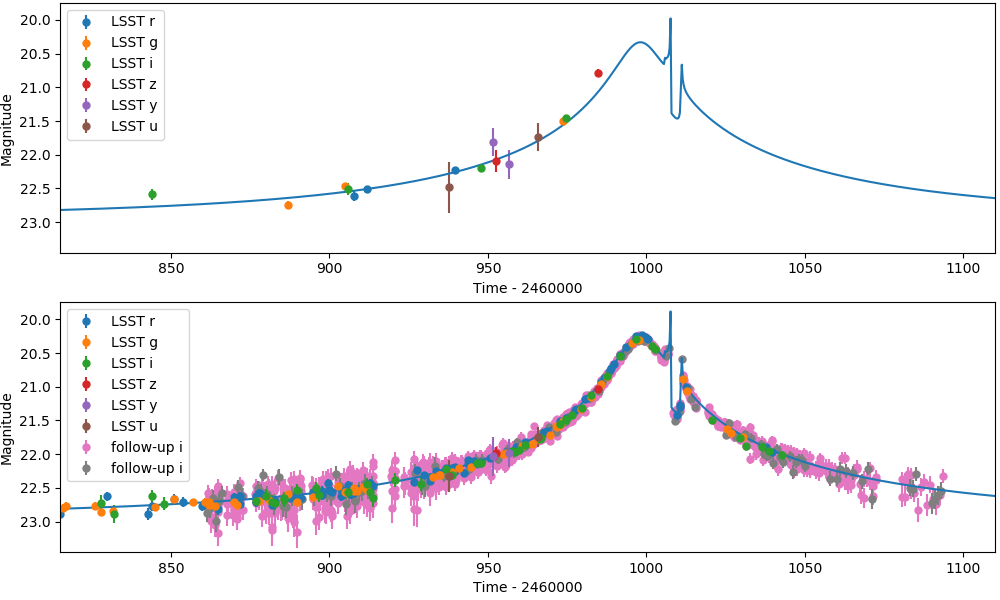
\includegraphics[width=\textwidth]{plot_1}
 \caption{Example light curves of a planetary microlensing event. 
{\it Upper panel} shows light curve in {\tt baseline\_2018a} OpSim run.  
{\it Lower panel} shows light curve with enhanced coverage as proposed here. 
}
\end{figure}

\begin{figure}[p]
 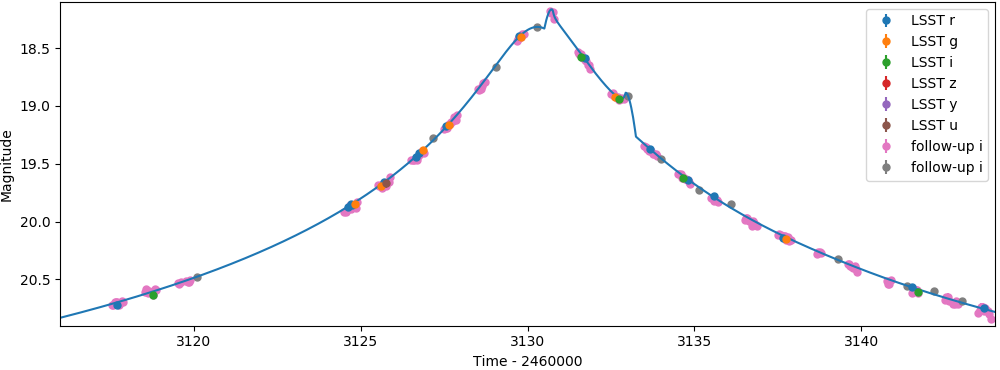
\includegraphics[width=\textwidth]{plot_2}
 \caption{Example light curve of a high-magnification planetary microlensing event. 
} 
\end{figure}



\section{Technical Description}
%\begin{footnotesize}
%{\it Describe your survey strategy modifications or proposed observations. Please comment on each observing constraint
%below, including the technical motivation behind any constraints. Where relevant, indicate
%if the constraint applies to all requested observations or a specific subset. Please note which 
%constraints are not relevant or important for your science goals.}
%\end{footnotesize}

% NO CONTENT HERE - ONLY IN SUBSECTIONS


\subsection{High-level description}
%\begin{footnotesize}
% XXX {\it Describe or illustrate your ideal sequence of observations.}
%\end{footnotesize}

{\bf Here we present technical description of a program where LSST 
sampling is sufficient to discover microlensing events in the SMC, 
while most of planet sensitivity comes from the follow-up observations.  
If most of planet sensitivity comes from the LSST observations, 
then the cadence would need to be improved to 1 hour.  
}

We propose for on the order of 2000 visits
to be taken each of two fields in the center of SMC.  
The sampling should be uniform in time and $r$, $g$, and $i$ 
filters give the highest yield.

\subsection{Footprint -- pointings, regions and/or constraints}
%\begin{footnotesize}{\it Describe the specific pointings or general region (RA/Dec, Galactic longitude/latitude or 
%Ecliptic longitude/latitude) for the observations. Please describe any additional requirements, especially if there
%are no specific constraints on the pointings (e.g. stellar density, galactic dust extinction).}
%\end{footnotesize}

The large field of view of LSST allows covering almost the entire sky-region 
of interest in two pointings centered at (${\rm R.A.}, {\rm Dec.}$) of 
$(17.58^{\circ}, -72.40^{\circ})$ and 
$(9.62^{\circ}, -73.82^{\circ})$.  
These fields were selected with constrained that their separation is similar to 
separations of fields in {\tt baseline\_2018a} OpSim run. 
If single pointing is chosen, then it should be placed at
$(14.50^{\circ}, -73.00^{\circ})$.  

\subsection{Image quality}
%\begin{footnotesize}{\it Constraints on the image quality (seeing).}\end{footnotesize}

Due to high crowding of the field, we request observations with seeing $< 2~{\rm arcsec}$.


\subsection{Individual image depth and/or sky brightness}
%\begin{footnotesize}{\it Constraints on the sky brightness in each image and/or individual image depth for point sources.
%Please differentiate between motivation for a desired sky brightness or individual image depth (as 
%calculated for point sources). Please provide sky brightness or image depth constraints per filter.}
%\end{footnotesize}

We request $r$ and $g$ band image depths of $\lesssim23.5~{\rm mag}$ 
and $i$ band depth of $\lesssim23.0~{\rm mag}$.  
The depths may be relaxed at the beginning and end of the SMC observing season 
in order to extend the time coverage each year, during which the data are collected.

The SMC is located far from Ecliptic, hence, it can be observed 
independently of the Moon phase.


\subsection{Co-added image depth and/or total number of visits}
%\begin{footnotesize}{\it  Constraints on the total co-added depth and/or total number of visits.
%Please differentiate between motivations for a given co-added depth and total number of visits. 
%Please provide desired co-added depth and/or total number of visits per filter, if relevant.}
%\end{footnotesize}

The high detection efficiency of microlensing events requires a uniform sampling and
a cadence on the order of $1~{\rm day}$.  This translates to on the order of
2000 epochs % XXX
after accounting for visibility and weather constraints.

There is no direct constraint on the co-added image depth.


\subsection{Number of visits within a night}
%\begin{footnotesize}{\it Constraints on the number of exposures (or visits) in a night, especially if considering sequences of visits.  }
%\end{footnotesize}

The optimal strategy is to take one or two epochs per night.  
If there are multiple visits during one night, 
then they should be separated by at least 1~hour.


\subsection{Distribution of visits over time}
%\begin{footnotesize}{\it Constraints on the timing of visits --- within a night, between nights, between seasons or
%between years (which could be relevant for rolling cadence choices in the WideFastDeep. 
%Please describe optimum visit timing as well as acceptable limits on visit timing, and options in
%case of missed visits (due to weather, etc.). If this timing should include particular sequences
%of filters, please describe.}
%\end{footnotesize}

The detection of microlensing events is best done with a uniform sampling.  
We request higher cadence at the beginning of the survey 
(until at least $>15$ epochs are collected in $r$, $g$, and $i$ bands), 
because microlensing events can be found only after establishing, 
which stars are constant.  In order to achieve a uniform cadence, 
it may be necessary to observe the field at airmass as large as $2.0$.


\subsection{Filter choice}
%\begin{footnotesize}
%{\it Please describe any filter constraints not included above.}
%end{footnotesize}

The number of observable sources is the largest in the $r$ band.  
The slightly smaller number of visible sources is in the $g$ band, and 
the third best filter is $i$.  Hence, we request 
the relative number of epochs to be $4:2:1$ in $r$, $g$, and $i$ bands, respectively.  
Having multi-band observations is important in order to characterize 
the properties of sources in microlensing events. % XXX ref

\subsection{Exposure constraints}
%\begin{footnotesize}
%{\it Describe any constraints on the minimum or maximum exposure time per visit required (or alternatively, saturation limits).
%Please comment on any constraints on the number of exposures in a visit.}
%\end{footnotesize}

We request standard $2\times15~{\rm s}$ or $1\times30~{\rm s}$ visits.  
The total exposure time per visit is constrained by the desired depth of a single visit.  
Saturation of the brightest objects is not an issue, because there are almost 
no events with sources saturated in standard LSST visits and if an event 
becomes brighter than the saturation limit, then the follow-up resources 
will provide an adequate photometric coverage.


\subsection{Other constraints}
%\begin{footnotesize}
%{\it Any other constraints.}
%\end{footnotesize}

% XXX
There are no other constraints.


\subsection{Estimated time requirement}
%\begin{footnotesize}
%{\it Approximate total time requested for these observations, using the guidelines available at \url{https://github.com/lsst-pst/survey_strategy_wp}.}
%\end{footnotesize}

The exposure time ($30~{\rm s}$) plus shutter open/close is  
$32~{\rm s}$.  The slew time is going to be relatively short.  The closest field 
that is observed with the standard Wide-Fast-Deep cadence in {\tt baseline\_2018a} 
is separated by only $11^{\circ}$.  
More importantly, one of the Deep Drilling fields (namely 
${\rm R.A.} = 23.29^{\circ}$, 
${\rm Dec.} = -63.32^{\circ}$) is located only $13^{\circ}$ away.  
Observations of this Deep Drilling field give many chances to slew to 
the SMC fields without too much overhead on slew and filter change.  
We estimate that typical slew and settle time will be $15~{\rm s}$ 
for the first field and $5~{\rm s}$ for the second field.  
We also estimate that a quarter of the visits will require filter change, which takes $120~{\rm s}$.  
The average total time of a visit in both fields is thus 
$120~{\rm s}/4 + 15~{\rm s} + 32~{\rm s} + 5~{\rm s} + 32~{\rm s} = 114~{\rm s}$.  
The total time requested for 2000 visits is only $63.33~{\rm h}$ or 
$0.26\%$ of the total time available ($24236~{\rm h}$).  
If only a single field is observed, then these numbers are 
$77~{\rm s}$, $42.78~{\rm h}$, and $0.18\%$, respectively. 

\begin{table}[ht]
    \centering
    \begin{tabular}{l|l}
        \toprule
        Properties & Importance \hspace{.3in} \\
        \midrule
        Image quality &  2 \\
        Sky brightness &  3 \\
        Individual image depth & 1  \\
        Co-added image depth &  3 \\
        Number of exposures in a visit   &  3 \\
        Number of visits (in a night)  &  1 \\ 
        Total number of visits &  1 \\
        Time between visits (in a night) & 2 \\
        Time between visits (between nights)  &  1 \\
        Long-term gaps between visits & 3 \\
        Other (please add other constraints as needed) & 3 \\
        \bottomrule
    \end{tabular}
     \caption{{\bf Constraint Rankings:} Summary of the relative importance of various survey strategy constraints. Please rank the importance of each of these considerations, from 1=very important, 2=somewhat important, 3=not important. If a given constraint depends on other parameters in the table, but these other parameters are not important in themselves, please only mark the final constraint as important. For example, individual image depth depends on image quality, sky brightness, and number of exposures in a visit; if your science depends on the individual image depth but not directly on the other parameters, individual image depth would be `1' and the other parameters could be marked as `3', giving us the most flexibility when determining the composition of a visit, for example.}
         \label{tab:obs_constraints}
\end{table}

\subsection{Technical trades}
%\begin{footnotesize}
%{\it To aid in attempts to combine this proposed survey modification with others, please address the following questions:
\begin{footnotesize}
\begin{enumerate}
    \item[1.] What is the effect of a trade-off between your requested survey footprint (area) and requested co-added depth or number of visits?
\end{enumerate}
\end{footnotesize}

We request observations of two fields.  If only a single optimally-placed field is observed 
with the same cadence, then the figure of merit presented below decreases by $19\%$.  

There is no direct constraint on the co-added depth. 

\begin{footnotesize}
\begin{enumerate}
    \item[2.] If not requesting a specific timing of visits, what is the effect of a trade-off between the uniformity of observations and the frequency of observations in time? e.g. a `rolling cadence' increases the frequency of visits during a short time period at the cost of fewer visits the rest of the time, making the overall sampling less uniform.
\end{enumerate}
\end{footnotesize}

The uniform cadence is requested and is most advantageous for the proposed 
science program.  The increase of visit frequency (at the cost of lower 
frequency at other times) will only help if short-lasting caustic-crossing 
features are predicted, but in those cases the follow-up resources should be used, not LSST.

\begin{footnotesize}
\begin{enumerate}
    \item[3.] What is the effect of a trade-off on the exposure time and number of visits (e.g. increasing the individual image depth but decreasing the overall number of visits)?
\end{enumerate}
\end{footnotesize}

A decrease in overall number of visits is not desirable, because it will delay 
the detection of the microlensing events.  It will allow additional very faint 
events to be observed, but their value will be lower due to the limited depth of 
the follow-up observations. 

\begin{footnotesize}
\begin{enumerate}
    \item[4.] What is the effect of a trade-off between uniformity in number of visits and co-added depth? Is there any benefit to real-time exposure time optimization to obtain nearly constant single-visit limiting depth?
\end{enumerate}
\end{footnotesize}

Only two fields are proposed here and a uniform sampling in time is more 
important than uniform depth of each visit.

\begin{footnotesize}
\begin{enumerate}
    \item[5.] Are there any other potential trade-offs to consider when attempting to balance this proposal with others which may have similar but slightly different requests?
\end{enumerate}
\end{footnotesize}

We expect that there will be other proposals that request observations of the SMC and LMC 
\citep[see Sec.~7 in][]{marshall17}.  Most of the other proposals will probably 
put stronger requests on observing a large area of the Clouds at the expense of lower cadence.  
Our proposal is most beneficial at the center of SMC.  We expect variability 
studies in the SMC (including planetary transits) will be optimized towards 
the largest number of stars monitored, which is in accordance with the plan 
proposed here. Observations in $u$, $z$, and $y$ bands may be requested 
in other proposals, but these bands have low value for the science program 
proposed here.  If observations in $u$, $z$, and $y$ bands 
are executed in addition to our program, then they 
will improve the source characterization to a small degree.  
If a wide area around the center of the SMC is proposed in other proposals 
than combining these observations with our program will lower the overheads. 


% \clearpage
% \vspace{.6in}

\section{Performance Evaluation}
%\begin{footnotesize}
%{\it Please describe how to evaluate the performance of a given survey in achieving your desired
%science goals, ideally as a heuristic tied directly to the observing strategy (e.g. number of visits obtained
%within a window of time with a specified set of filters) with a clear link to the resulting effect on science.
%More complex metrics which more directly evaluate science output (e.g. number of eclipsing binaries successfully
%identified as a result of a given survey) are also encouraged, preferably as a secondary metric.
%If possible, provide threshold values for these metrics at which point your proposed science would be unsuccessful 
%and where it reaches an ideal goal, or explain why this is not possible to quantify. While not necessary, 
%if you have already transformed this into a MAF metric, please add a link to the code (or a PR to 
%\href{https://github.com/lsst-nonproject/sims_maf_contrib}{sims\_maf\_contrib}) in addition to the text description. (Limit: 2 pages).}
%\end{footnotesize}

% XXX  - (Limit: 2 pages)

To evaluate performance of particular observing strategy 
in achieving our science goals, we propose {\bf figure of merit} (FoM), 
which is a number of SMC planets discovered.  The number is evaluated 
assuming a fiducial planet frequency and taking into account the follow-up
observations, as described below.  We provide software that evaluates 
FoM based on OpSim simulation.  This software is not part of MAF package.  
Evaluating FoM for a single OpSim simulation with accuracy of $5\%$ 
takes about $6~{\rm h}$.  

In our simulations of detection efficiency, 
we have included intensive photometric follow-up observations.  
The optimum follow-up would be a uniform and 24-hour coverage of 
every on-going microlensing event with a high photometric accuracy. 
The SMC lies close to the South celestial pole and there is a limited number of 
observatories with good astronomical climate that can observe the SMC.  
There is a number of telescopes located in Chile, but they cover a narrow 
range of longitudes.  Outside Chile, the only observatories with large aperture telescopes are 
Siding Spring Observatory (Australia) and 
South African Astronomical Observatory (South Africa).  
The number of clear nights and seeing are better for Chilean observatories.  
Taking all these aspects into account, we divide the follow-up observations 
into Chilean and non-Chilean.  
For Chilean observatories, we assume observations are taken when the SMC center 
is at the altitude $>30^{\circ}$ and Sun is at the altitude $<-15^{\circ}$ 
as seen from Cerro Pach\'{o}n.  We select nights for which these conditions 
are fulfilled for at least $30~{\rm min}$ and assume uniform cadence of 
$1~{\rm h}$.  To simulate the impact of clouds, we remove epochs for which 
there is no LSST observations (in any field) $1~{\rm h}$ prior or after 
considered follow-up epoch.  There are in total ten optical telescopes 
in Chile that have aperture of $4~{\rm m}$ or larger.  
We assume that follow-up observations will be conducted 
using a $\approx4$-${\rm m}$ aperture telescope and the same exposure time as for LSST.  
The same photometric accuracy should be achievable using longer (and still reasonable) 
exposure times on a 2-m class telescopes.  To account for airmass, seeing, and 
sky transparency on photometric accuracy, we use the accuracy of the closest 
LSST observation with additional correction of $\delta m_5 = -0.53~{\rm mag}$ 
added to $5\sigma$ depth of LSST (for this we use the $i$-band observations 
in a few fields close to SMC), see \citet{ivezic18}. 

The potential follow-up telescopes outside Chile have smaller apertures and 
poorer weather conditions.  We simulate these additional follow-up epochs 
assuming there is a single epoch per night and it is shifted by 12~h 
relative to observations in Chile.  Additionally, we select half of 
the nights only.  To estimate photometric accuracy of these data, we follow 
the same procedure as for Chilean follow-up observations. 
For each event, the follow-up observations are assumed to start $12~{\rm h}$ 
after the event detection and end $3t_{\rm E}$ after the event peaks.

The above strategy leads to on average 1400 follow-up epochs for 
Chilean observatories over 10-month long season in {\tt baseline\_2018a} run. 
For non-Chilean observatories there are on average 120 follow-up 
epochs per season.  

We simulate planetary systems assuming the planet frequency 
as derived from recent microlensing studies in Galactic bulge fields:
\citet{suzuki16} and \citet{udalski18b}.  The planet frequency 
is a function of microlensing parameters: 
mass ratio $q$ and projected separation $s$.
For the SMC events, the Einstein ring radius is smaller than for bulge events, 
but the lens is at larger distance, and these two effects approximately cancel out.  
As a result, the values of $s$ in the SMC that are probed by microlensing are similar 
to the values in the Galactic bulge fields.  % XXX
We may expect that planet frequency is lower in the SMC, but for 
calculating the FoM, we assume the same as in the Galactic bulge 
and request sampling that leads to at least a few planets discovered under this assumption. 

To evaluate the FoM, we multiply the number of microlensing events 
in the monitored sky-area over the survey time-span 
by the fraction of events that show planetary 
anomalies with significance $\Delta\chi^2>100$.  This fraction depends 
on input from OpSim.  To estimate the number of events, 
we multiply event rate in sky-area considered ($2.7\times10^{-7}~{\rm yr^{-1}}$), 
the total number of sources in the SMC ($1.7\times10^{9}$), 
the fraction of sources that are in monitored area ($0.67$), 
the fraction of sources in brightness range detectable with LSST ($0.098$), and 
the survey time-span ($10~{\rm yr}$).  This results in $293$ events.  
We simulated an observing strategy that follows our request 
and estimated the fraction of events that show detectable planetary 
anomalies to be $0.0097$.  Hence, the expected planet yield is $2.84$.  
% XXX add value for baseline_2018a
The threshold value of our FoM (at which point proposed science would be unsuccessful) 
is $2.5$ and the ideal goal is $4.0$. 

The software for evaluating FoM is available at:
\begin{center}
\url{https://github.com/rpoleski/LSST_SMC}
\end{center}


\vspace{.6in}

\section{Special Data Processing}
%\begin{footnotesize}
%{\it Describe any data processing requirements beyond the standard LSST Data Management pipelines and how these will be achieved.}
%\end{footnotesize}

Standard photometric data processing of LSST data will be enough.  
There are several implementations of algorithms that find 
the microlensing events in large datasets.  Also the algorithms for 
scheduling observations of follow-up telescopes have been implemented.  
We will build a dedicated pipeline that incorporates solutions from previous 
observing campaigns. 


%  \section{Acknowledgements}  XXX

\section{References}

\newcommand*\aap{A\&A}
\let\astap=\aap
\newcommand*\aapr{A\&A~Rev.}
\newcommand*\aaps{A\&AS}
\newcommand*\actaa{Acta Astron.}
\newcommand*\aj{AJ}
\newcommand*\ao{Appl.~Opt.}
\let\applopt\ao
\newcommand*\apj{ApJ}
\newcommand*\apjl{ApJ}
\let\apjlett\apjl
\newcommand*\apjs{ApJS}
\let\apjsupp\apjs
\newcommand*\aplett{Astrophys.~Lett.}
\newcommand*\apspr{Astrophys.~Space~Phys.~Res.}
\newcommand*\apss{Ap\&SS}
\newcommand*\araa{ARA\&A}
\newcommand*\azh{AZh}
\newcommand*\baas{BAAS}
\newcommand*\bac{Bull. astr. Inst. Czechosl.}
\newcommand*\bain{Bull.~Astron.~Inst.~Netherlands}
\newcommand*\caa{Chinese Astron. Astrophys.}
\newcommand*\cjaa{Chinese J. Astron. Astrophys.}
\newcommand*\fcp{Fund.~Cosmic~Phys.}
\newcommand*\gca{Geochim.~Cosmochim.~Acta}
\newcommand*\grl{Geophys.~Res.~Lett.}
\newcommand*\iaucirc{IAU~Circ.}
\newcommand*\icarus{Icarus}
\newcommand*\jcap{J. Cosmology Astropart. Phys.}
\newcommand*\jcp{J.~Chem.~Phys.}
\newcommand*\jgr{J.~Geophys.~Res.}
\newcommand*\jqsrt{J.~Quant.~Spectr.~Rad.~Transf.}
\newcommand*\jrasc{JRASC}
\newcommand*\memras{MmRAS}
\newcommand*\memsai{Mem.~Soc.~Astron.~Italiana}
\newcommand*\mnras{MNRAS}
\newcommand*\na{New A}
\newcommand*\nar{New A Rev.}
\newcommand*\nat{Nature}
\newcommand*\nphysa{Nucl.~Phys.~A}
\newcommand*\pasa{PASA}
\newcommand*\pasj{PASJ}
\newcommand*\pasp{PASP}
\newcommand*\physrep{Phys.~Rep.}
\newcommand*\physscr{Phys.~Scr}
\newcommand*\planss{Planet.~Space~Sci.}
\newcommand*\pra{Phys.~Rev.~A}
\newcommand*\prb{Phys.~Rev.~B}
\newcommand*\prc{Phys.~Rev.~C}
\newcommand*\prd{Phys.~Rev.~D}
\newcommand*\pre{Phys.~Rev.~E}
\newcommand*\prl{Phys.~Rev.~Lett.}
\newcommand*\procspie{Proc.~SPIE}
\newcommand*\qjras{QJRAS}
\newcommand*\rmxaa{Rev. Mexicana Astron. Astrofis.}
\newcommand*\skytel{S\&T}
\newcommand*\solphys{Sol.~Phys.}
\newcommand*\sovast{Soviet~Ast.}
\newcommand*\ssr{Space~Sci.~Rev.}
\newcommand*\zap{ZAp}
\def\arxivprefixesep{:}
\newcommand{\eprint}[2][]{{\tt\if!#1!#2\else#1\arxivprefixesep\ignorespaces#2\fi}}

\renewcommand{\bibsection}{}

\bibliographystyle{aa}
\bibliography{SMC_LSST}

\end{document}
